\section{Aufgabe1}
\label{sec:Aufgabe1}
%\lstinputlisting[language=Python, firstline=15, lastline=21]{plots/plot.py}
\subsection{Teilaufgabe a)}
Um die $10^5$ Signalereignisse mit der Transformationsmethode zu gernerieren werden
mit
\begin{equation*}
  E=(1-x)^{\frac{-1}{1,7}}
\end{equation*}
die Energieereignisse gesamplet. Die dazugehörige Rechnung befindet sich auf dem
seperat abgegebenen Zettel.
\subsection{Teilaufgabe b)}
Mit dem Neumann'schen Rückweisungsverfahren wurden die tatsächlich detektierten
Ereignisse gesamplet. Das Ergebnis ist in Abbildung \ref{fig:Energie} dargestellt.
\begin{figure}[h]
  \centering
  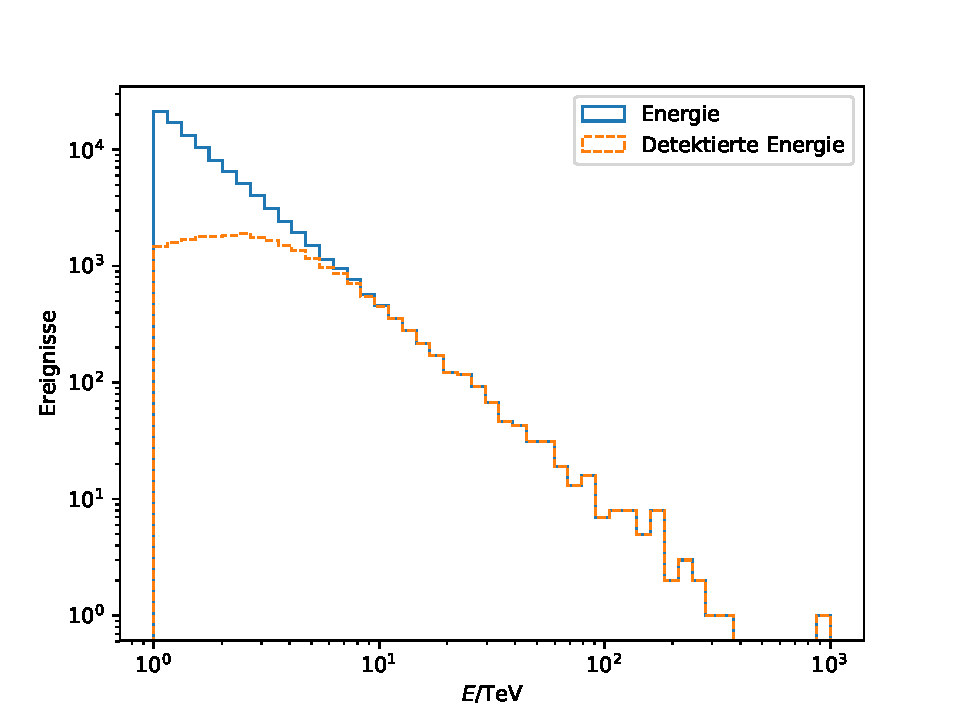
\includegraphics[height = 8cm]{plots/Energie.pdf}
  \caption{Energieereignisse und tatsächlich detektierte Energieereignisse.}
  \label{fig:Energie}
\end{figure}
\subsection{Teilaufgabe c)}
Die Anzahl der angesprochenen Photomultiplier (Hits) werden aus einer Normalverteilung
mit $\mu=10 E$ und $\sigma=2 E$ ($E$ in TeV) gezogen. Dabei gehen nur
die Energien der detektierten Ereignisse ein. Dies sind von den Anfangs $10^5$ Werten noch
etwa $25000$ Werte.
\subsection{Teilaufgabe d)}
Die Ortsmessung ist Abhängig von der Anzahl an Hits und damit wiederum Energieabhängig.
Das Signal trifft am Punkt (7, 3) auf den quadratische Detektor. Für die x- und y-Richtung
wird eine Normalverteilung angenommen mit $\sigma=(\log_{10}(N+1))^{-1}$.
Das Ergebnis ist in dem 2D-Histogramm \ref{fig:Ort} aufgetragen.
\begin{figure}[h]
  \centering
  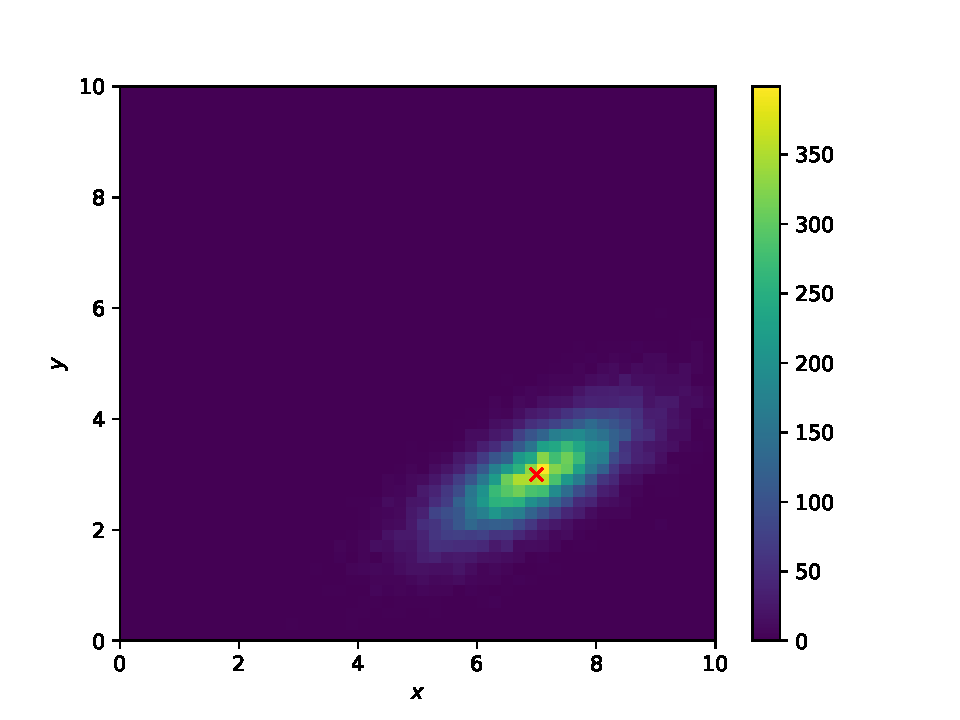
\includegraphics[height = 8cm]{plots/Ort.pdf}
  \caption{Darstellung der Ortsmessung.}
  \label{fig:Ort}
\end{figure}
Dabei wurden jeweils 50 Bins in die beiden Richtungen gewählt.
\subsection{Aufgabenteil e)}
Die hier gezeigten Berechnungen sind mit nur $10^5$ Untergrund-Ereignissen durchgeführt,
da die verwendete Funktion für die Ortsauflösung laufzeitungünstig geschrieben ist. Mit $10^7$ Ereignissen würde das Programm ca.
370 Stunden laufen. Leider hatte ich nicht mehr die Zeit die Funktion sinnvoll umzuschreiben.
\begin{figure}[h]
  \centering
  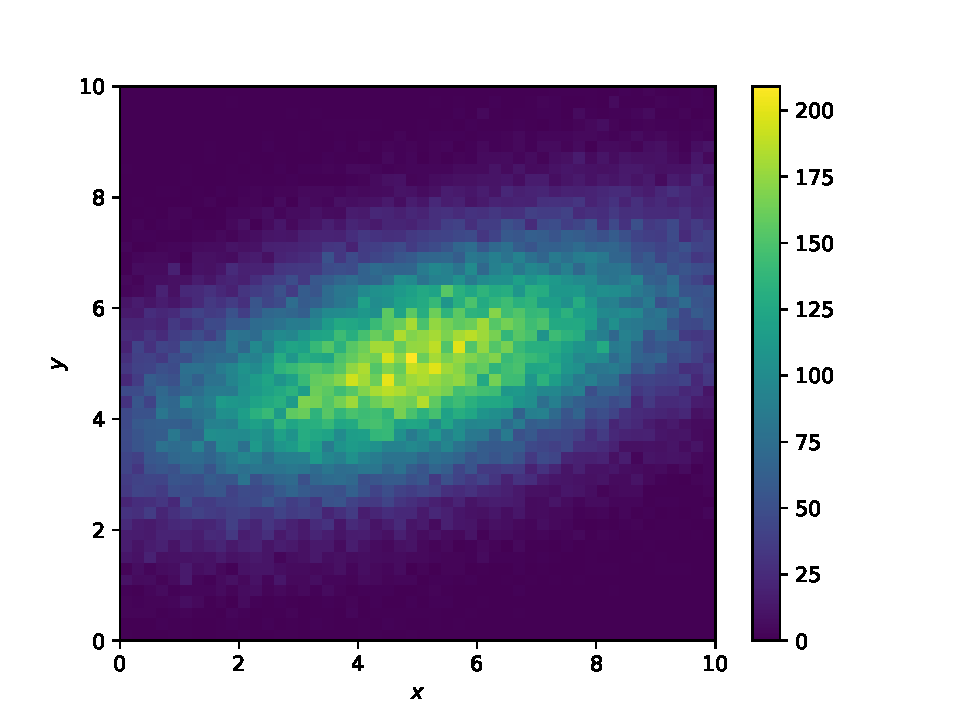
\includegraphics[height = 8cm]{plots/Ort_BKG.pdf}
  \caption{Darstellung der Ortsmessung für den Untergrund.}
  \label{fig:Ort_BKG}
\end{figure}
\begin{figure}[h]
  \centering
  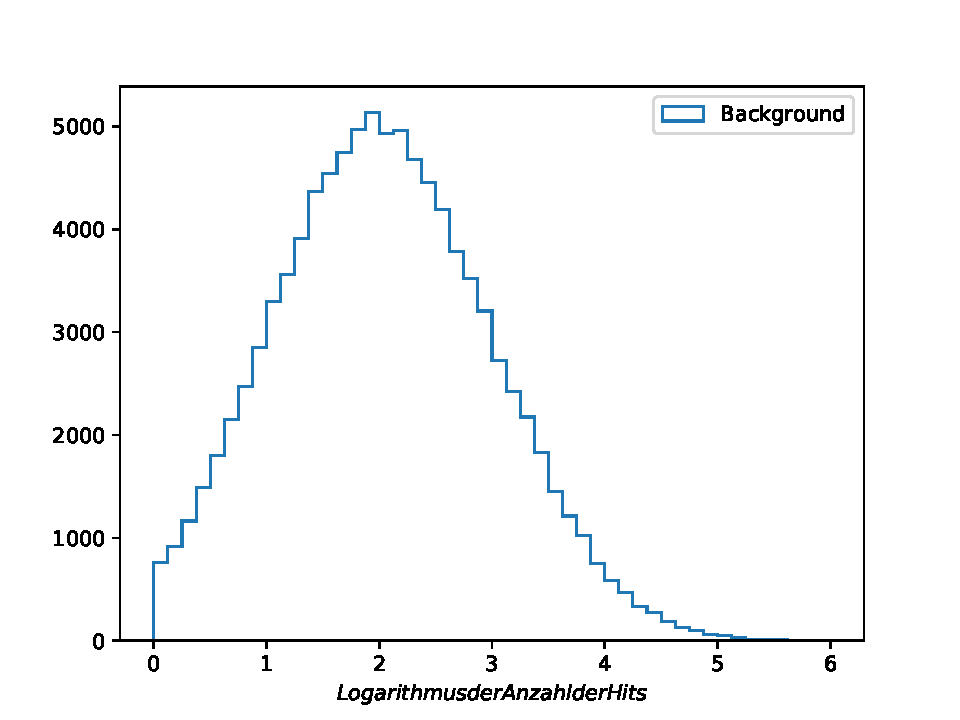
\includegraphics[height = 8cm]{plots/Hits_BKG.pdf}
  \caption{Darstellung der Untergrund-Hits.}
  \label{fig:Hits_BKG}
\end{figure}
